\section{Proceso Operativo SIGCSA-PO-14}
\par 

	El objetivo de este proceso es de establecer y definir las instrucciones a seguir para realizar procesos de calibración de termómetros
	por comparación en baños isotérmicos de temperatura controlada, tomando en cuenta todas las
	recomendaciones del fabricante.
	
\subsection{Alcance}
\par 
	Para ser aplicado en Bancos de Sangre y Laboratorios que tengan termómetros de vidrio o digitales
	como instrumentos para el monitoreo de temperatura.
	
\subsection{Disposiciones Generales}
\subsubsection{Inspección Visual}

\begin{itemize}
	\item Bulbo: Verifique que no exista presencia de algún material extraño, ruptura o
	raspadura.
	
	\item Columna Capilar: Verifique que no exista ruptura o raspadura del capilar que
	impida visualizar la columna de líquido, deformación, presencia de algún material
	extraño.
	
	\item Columna de Líquido: Verifique que no exista oxidación en el caso de termómetros
	de mercurio.
	
	\item Cámara de Expansión y de Contracción: Verifique que no exista presencia de algún
	material extraño.
	
	\item Pantalla Digital: Verifique que no exista ruptura (termómetros digitales).
	
	\item Sonda/Sensor de Temperatura: Verifique no exista ruptura, degradación o
	desgaste.
	
	\item Baterías: Verifique el correcto estado de las baterías (termómetros digitales).
\end{itemize}
		
\subsubsection{Método de Calibración por Comparación Directa}

\par 
	Consiste en colocar el termómetro patrón con los termómetros a calibrar en el baño
	termostático o punto de referencia física, bajo condiciones que permitan que los
	sensores de cada uno de ellos alcancen una temperatura estable. La toma de lecturas
	debe iniciarse cuando se asegure que la temperatura de los termómetros ha alcanzado
	un valor estable\cite{po14}.
\subsubsection{Condiciones Para la Calibración}

\par 
	El ensayo debe realizarse a una temperatura promedio de 20±5ºC y una humedad
	relativa no mayor a 80\%. El equipo a calibrar debe mantenerse en el lugar de la
	calibración en posición vertical por un lapso de tiempo no menor a 1 hora\cite{po14}.
	
\subsubsection{Equipos e Instrumentación \cite{po14}}

\begin{itemize}
	\item Termómetro certificado
	\item Termohigrómetro certificado
	\item Baño Termostático
\end{itemize}

\subsection{Análisis}

\begin{itemize}
\item Documentación Inicial: En este paso se anotan todos los parametros de las condiciones ambientales y otras disposiciones generales para validad que el procedimiento sea valido.

\item Instalación: Se elabora o se inicia el punto de referencia fisica para poder empezar la calibración. Una vez el punto de referencia llega a la temperatura deseada se coloca el termómetro patron y el termómetro a calibrar en el punto de referencia y se espera a la estabilización de las temperaturas.

\item Captura de datos: Se documenta la temperatura enseñada en ambos termómetros cada minuto por 10 minutos. Al finalizar se documenta la temperatura y la humedad del ambiente.

\item Calculo del Error: Se determina el error del termómetro a calibrar con respecto al termómetro patrón. Un error aceptable es no mayor a 1ºC.
\end{itemize}

\begin{figure}[H]
	\centering
	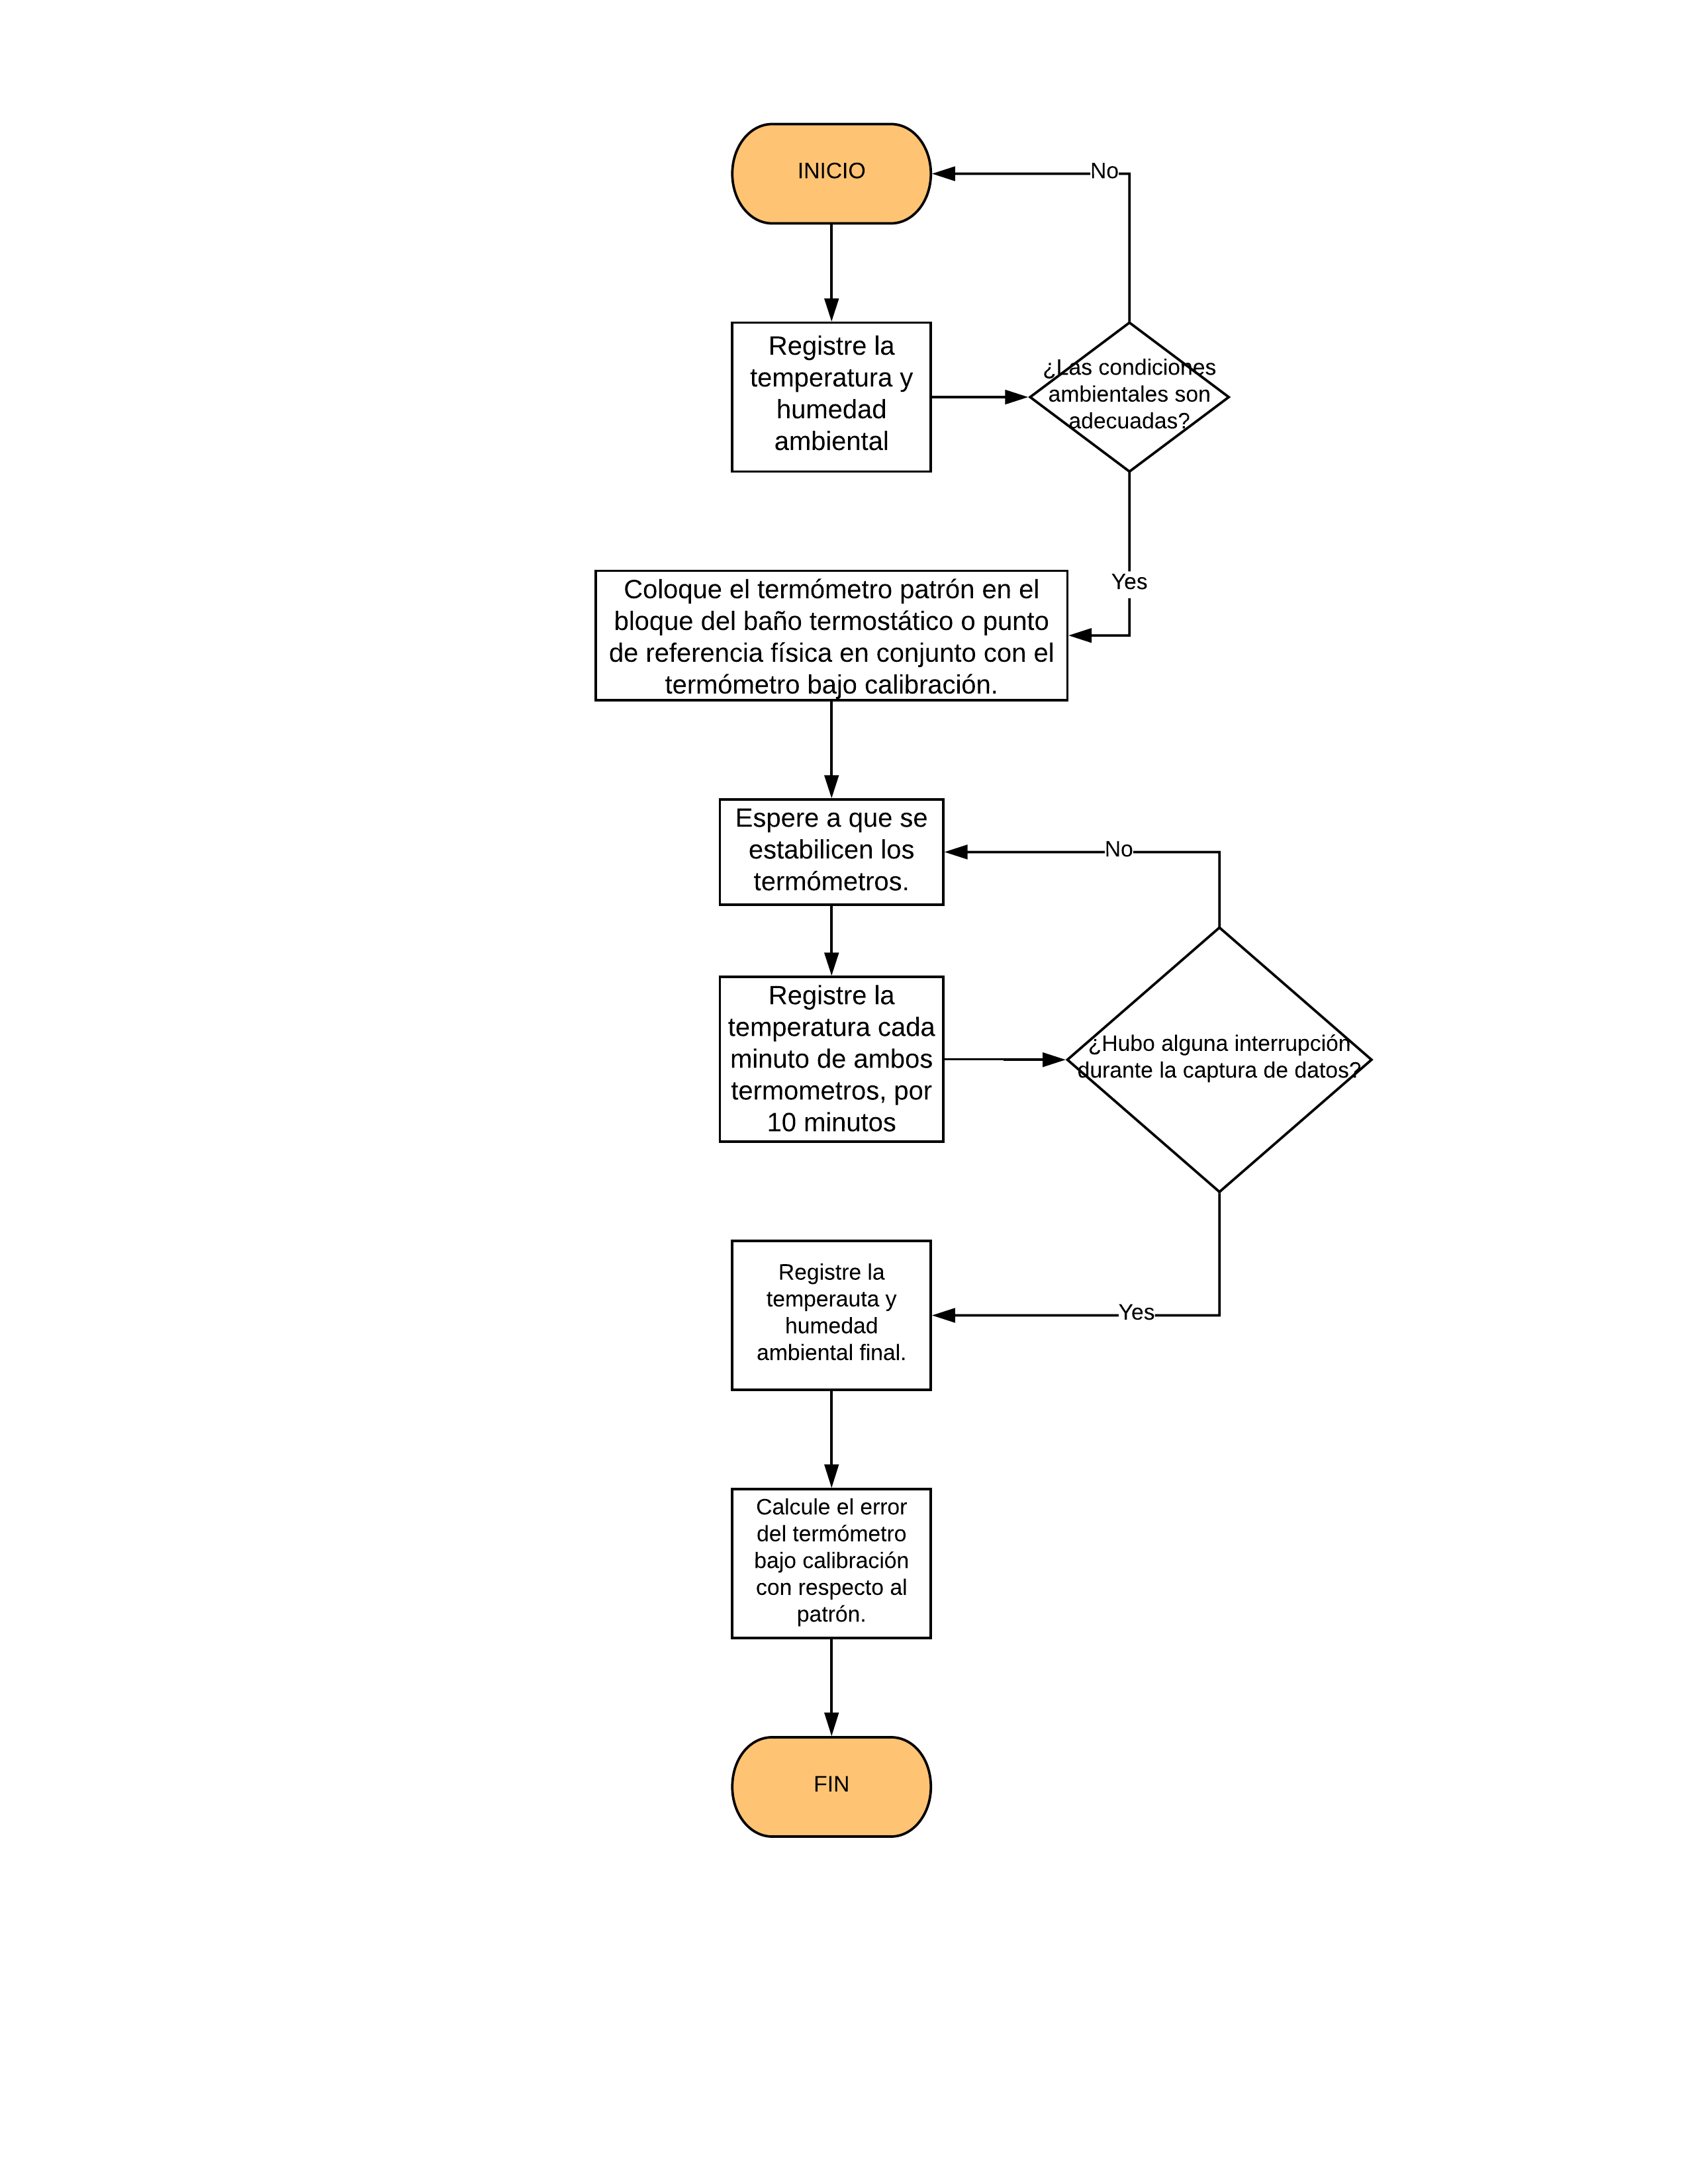
\includegraphics[width=\textwidth]{diagram2.png}
	\caption{Diagrama de Flujo del proceso operativo SIGCSA-PO-14}
\end{figure}